\documentclass[a4paper, parskip=full]{scrartcl}
\usepackage[top=3cm, bottom=3.5cm, left=3cm, right=3cm]{geometry}
\usepackage[utf8]{inputenc} % use utf8 file encoding for TeX sources
\usepackage[LGR,T1]{fontenc}    % avoid garbled Unicode text in pdf
\usepackage[german]{babel}  % german hyphenation, quotes, etc
\usepackage{graphicx}       % provides commands for including figures
\usepackage{csquotes}       % provides \enquote{} macro for "quotes"
\usepackage{hyperref}       % detailed hyperlink/pdf configuration
\usepackage{color}
\usepackage{tabu}			% provides tables
\usepackage[nonumberlist]{glossaries}     % provides glossary commands
\hypersetup{                % ‘texdoc hyperref‘ for options
  pdftitle={Pflichtenheft},
  pdfauthor={Anna Csurkó, Jona Enzinger, Yannik Schmid, Jonas Zoll},
}
\graphicspath{{./figures/}} % Setting the graphicspath

\newcounter{counter}[section]
\setcounter{counter}{10}

% new environment for listing requirements/product data/... with a counter
\newenvironment{Kriterien}[1]{
	\let\olditem\item \renewcommand\item[1][]{\olditem[/#1\thecounter /] \textbf{##1} \hfill \\
	\addtocounter{counter}{10}} \begin{description}}
	{\end{description}}


\title{Pflichtenheft}
\author{Anna Csurkó, Jona Enzinger, Yannik Schmid, Jonas Zoll}
\makeatletter

\definecolor{mintgreen}{RGB}{50,161,137} % theme color of the Karlsruhe Institute of Technology (KIT)

% header and footer
\usepackage[automark,autooneside=false,headsepline=0.5pt,footsepline=0.5pt]{scrlayer-scrpage}
\addtokomafont{headsepline}{\color{mintgreen}}
\addtokomafont{footsepline}{\color{mintgreen}}
\addtokomafont{pagehead}{\normalfont}

% delete current settings for header and footer
\clearpairofpagestyles

% display document name on the left and current section on the right
\ihead{\@title}
\ohead{\rightmark}

% center page number
\cfoot*{\pagemark}

% load glossary entries
\makenoidxglossaries
\loadglsentries{./chapters/Glossareintraege}

\begin{document}
% beginn content
\begin{titlepage}
  \centering
  
\includegraphics[width=0.5\linewidth]{KITLogo.png}\par\vspace{1cm}
	  {\scshape \bfseries Lehrstuhl für Pervasive Computing Systems\par}
	  {\scshape \bfseries Teco\par}
	  \vspace{0.25cm}
  	{\scshape Tobias Röddiger\\Dr. Paul Tremper\par}
  	\vspace{1.5cm}

    \newcommand{\HRule}{\rule{\linewidth}{0.5mm}}
    {\color{mintgreen}\HRule} \\[0.4cm]
  	{\huge \bfseries \LARGE Anwenderorientierte Nutzerschnittstelle für Luftqualitätsdaten\par}
    {\color{mintgreen}\HRule} \\[1cm]
  	\vspace{2cm}
  	{\scshape \Large Anna Csurkó\\Jona Enzinger\\Yannik Schmid\\Jonas Zoll\par}
  	\vfill

\end{titlepage}


\tableofcontents
\section{Vorwort}
Dieses Dokument modelliert die Architektur des Programms \gls{SmartAQnet}. Wir als Entwickler-Team haben den Aufbau in Typescript components und Klassen aufgeteilt. Dabei war unser Ziel, das Programm möglichst stabil, flexibel und objektorientiert zu gestalten. Zusätzlich lässt sich die Architektur sehr gut in Model, View und Controller einteilen, indem wir die Querys, das Grundgerüst und die Benutzeroberfläche gut trennen können. Für die Erstellung der Diagramme wurde PlantUML und Visual Studio Code, für die Zusammenarbeit GitHub benutzt.


\section{Zielbestimmung}
Das erklärte Ziel der Anwendung ist es, Bürgern die Messdaten des \gls{SmartAQnet}-Projekts auf eine ansprechende Weise zugänglich zu machen.
Zu diesem Zweck wurde eine Befragung der Zielgruppe durchgeführt, auf deren Basis die angezeigten Informationen ausgewählt wurden.
Es sollen nicht die rohen \glspl{Messwert} im Mittelpunkt stehen sondern die Daten im verständlichen Kontext dargestellt werden.
Auch soll die Bedienung intuitiv ohne Eingewöhnungszeit möglich sein.
Die Anwendung soll die benötigten Daten selbstständig von einem \gls{FROST-Server} anfragen und, außer zur Übertragung der \gls{Webanwendung}, ohne \gls{Webserver} oder eigene Datenbank funktionieren.

\subsection{Musskriterien}
\setcounter{counter}{10}

\begin{Kriterien}{MK}

	\item \gls{Webanwendung}, lauffähig in allen modernen Browsern die JavaScript unterstützen

	\item Angepasste Layouts für Computer und \gls{Handy}
	
	\item Es können Anfragen in der \gls{Querysprache} des \gls{FROST-Server} erzeugt und übertragen werden.
	
	\item Die Antworten des \gls{FROST-Server} können in die benötigten Formen zur Anzeige umgewandelt werden.
	
	\item Aus den \glspl{Messwert} der verschiedenen Feinstaubgrößen kann ein einzelner \gls{Feinstaubindex} berechnet werden

	\item Eine interaktive Karte zeigt alle \glspl{Station} gleichzeitig. 
	
	\item Der Nutzer kann auswählen, welechen Ansicht die interaktive Karte anzeigen soll.
	
	\item Die Nutzer können Straßennamen und Stadtnamen eingeben und die interaktive Karte springt auf die Stelle. Es gibt eine Fehlermeldung, wenn der Ort nicht existiert.

	\item \glspl{Station} haben eine Färbung je nach Bewertung der \glspl{Messwert} auf der Skala.
	
	\item Beim Klicken auf eine \gls{Station} wird eine \gls{Pop-Up} Box angezeigt mit dem Name der Station, der Position und dem exakten Messwert.
		Über eine Schaltfläche kann die Detailansicht geöffnet werden. 
	
	\item Für jedes Feature wird ein Diagramm angezeigt, das die Entwicklung der \glspl{Messwert} zeigt. Die Zeitspanne ist einstellbar. Es werden nur Diagramme von Messwerten angezeigt, die an der \gls{Station} gemessen werden.
	
	\item Ein \gls{Graph} der die Veränderung von dem Tagesdurchschnitt anzeigt, dabei ist der Zeitabschnitt einstellbar.
	
	\item Es werden auch zusammengefasste Informationen angegeben: 
\end{Kriterien}
		
\begin{itemize}
	\item Wie viel Prozent die \glspl{Messwert} besser/schlechter sind als letztes Jahr.
    \item Vergleich mit Durchschnitt der \glspl{Messwert} im Umkreis.
    \item Der Feinstaubwert war an xxx Tagen größer als heute (mit \gls{Kuchendiagramm})
\end{itemize}

\begin{Kriterien}{MK}	
	\item Zur Karte zurückzukehren ist mit einem Klick möglich.
\end{Kriterien}

\newpage
\subsection{Wunschkriterien}
\setcounter{counter}{10}
\begin{Kriterien}{WK}

	\item Wechseln zwischen verschiedenen interaktiven Karten für die verschiedenen Aspekten der \glspl{Messwert}.

	\item Auf der Seite mit den Daten einer bestimmten \gls{Station} wird auf einer Karte gezeigt, wo die \gls{Station} sich befindet (nur für Desktop Layout). 

	\item Zusätzliche Informationen über die Zuverlässigkeit des Sensors sind erreichbar.

	\item Verschiedene Sprachen sind auswählbar (insbesondere Deutsch und Englisch)
	
	\item Auf der interaktiven Karte werden Städte als farbige Polygonen gekennzeichnet. Das Polygon ist nach dem Durchnitt in der Stadt gefärbt. Mit einem Klick auf das Polygon wird die Karte der Stadt angezeigt, auf der nur die Messtationen markiert sind. 
	
	\item Ein Diagramm  \gls{Graph} zeigt den Verlauf der \glspl{Messwert} Anzeigt und dabei auch den Durchschnitt markiert.
	
	\item Wenn der Nutzer GPS-Lokalisiernug erlaubt, startet die Karte beim jeden neuen Aufruf der Webanwendung an dem Wohnort des Nutzers.
	
	\item Die Webanwendung speichert, an welcher Stelle die interaktive Karte war, als der Nutzer die Detailansicht geöffnet hat, und öffnet beim Rückkehr wieder an der Stelle. Auch bei dem Wechsel zwischen den Features bleibt die Karte bei der gleichen Stelle und Größe.

\end{Kriterien}

\subsection{Abgrenzungskriterien}
\setcounter{counter}{10}
\begin{Kriterien}{AK}

	\item Historische Daten werden nicht einzeln angezeigt, nur die Diagramme geben Informationen.
	
	\item Die Seite gibt keine ausführliche Erklärung dazu, was genau die \glspl{Messwert} bedeuten, nur die daraus folgernde Luftqualität wird angezeigt. 
	
	\item Die Folgen und Ursachen der Feinstaubbelastung werden nicht genannt.
	
	\item Bei der Nutzung der \gls{Webanwendung} werden keine neue Tabs geöffnet. Alles passiert im gleichen Tab.
	
	\item Die \gls{Webanwendung} benutzt den Weberver nur um die Anwendung zu übertragen. 
		Es werden keine anderen Anfragen an den \gls{Webserver} gestellt.
	
	
\end{Kriterien}

\section{Produkteinsatz}

\subsection{Anwendungsbereiche}

Die \gls{Webanwendung} dient dafür dem Benutzer Informationen der \gls{SmartAQnet} Datenbank oder eines anderen \gls{FROST-Server} benutzerfreundlich darstellen zu lassen.

\subsection{Zielgruppen}

Benutzer der \gls{Webanwendung} sind interessierte Bürgerinnen und Bürger die sich über Luftqualitätsdaten informieren möchten. 
Dabei wird die \gls{Webanwendung} einfach gehalten um älteren Menschen, die im Umgang mit informationstechnischen Systemen noch nicht sehr erfahren sind, die Benutzung zu erleichtern.
Ob die Benutzer schon Kenntnisse im Bereich der Luftqualität haben, soll für die Benutzung der \gls{Webanwendung} unerheblich sein.

\subsection{Betriebsbedingungen}

Die \gls{Webanwendung} sollte rund um die Uhr und unbeaufsichtigt für prinzipiell unbeschränkt viele Benutzer zur Verfügung stehen, sofern der \gls{Webserver} auf dem die \gls{Webanwendung} läuft dies zulässt. 
Vorrausgesetzt für den Betrieb der \gls{Webanwendung} ist der Zugriff auf einen \gls{FROST-Server}.
\section{Produktumgebung}

\subsection{Software}

Der Benutzer benötigt einen aktuellen \gls{Webbrowser}.

\subsection{Hardware}

Für den Zugriff auf die \gls{Webanwendung} benötigt der Benutzer ein internetfähiges Gerät welches eine \gls{Webbrowser} ausführen kann.  
Die Bereitstellung der \gls{Webanwendung} erfordert außerderdem einen Server.
\section{Funktionale Anforderungen}

\setcounter{counter}{10}
\begin{Kriterien}{FA}

\subsection{Allgemeine Anforderungen}

 \item[Unterstützung mobile Endgeräte]
   Die \gls{Webanwendung} ist ohne jegliche Einschränkung auf mobilen Endgeräten nutzbar.  

 \item[Statische Webanwendung]
   Die \gls{Webanwendung} erfordert den \gls{Webserver} nur um die Anwendung zu übertragen.
   Sonst müssen keine Anfragen an den \gls{Webserver} gestellt werden. 

\subsection{Karte}

 \item[Startseite]
   Bei Aufrufen der Webseite wird die Startseite angezeigt.
   Es wird eine frei bewegliche Karte mit allen \glspl{Station} als \glspl{Pin} angezeigt und es kann nach einer Adresse gesucht werden.
   Ein Klick auf 'Ansicht' öffnet ein \gls{Pop-Up} mit Ansichten.

 \item[Stationen Pop-Up]
  Wird mit der Maus über einen Stations-\gls{Pin} gefahren/mit dem Finger darauf geklickt öffnet sich ein \gls{Pop-Up}.
  Darin werden der Name der \gls{Station}, die Koordinaten und den aktuellen exakten Messwerten angezeigt.
  Ein Klick auf 'Details anzeigen' öffnet die Detailansicht.

 \item[Ansichten]
   Die Karte auf der Startseite lässt sich über Ansichten anpassen.
   Es kann ausgewählt werden welche \glspl{Messwert} angezeigt werden.
   Es werden nur \glspl{Station} angezeigt die entsprechende Daten besitzen.
   Verschiedene Optionen zur Einfärbung der Karte und \glspl{Station} sind verfügbar.

 \item[Legende]
  Auf der Karte wird eine Legende angezeigt welche die aktuellen Einfärbungen erklärt.
  Dies kann beispielsweise durch eine Farbskala erfolgen.

 \item[Letzte Ansicht]
  Kehrt ein Nutzer zur Seite zurück wird die zuletzt genutzte Ansicht geladen.

 \subsubsection{Kartenansichten}

 \item[Standard]
  \glspl{Station} werden angezeigt und nach \glspl{Messwert} eingefärbt. 
  Überschrittene Grenzwerte werden zudem mit einem '!' markiert.

 \item[Flächenwerte (WK)]
   Zwischen den \glspl{Station} werden Dreiecke aufgespannt die entsprechend der Höhe der durchschnittlichen \glspl{Messwert} gefärbt werden.
   Dabei überschneiden sich die Dreiecke nicht.

 \item[Veränderung]
   Die \gls{Station} wird entsprechend der Veränderung über den letzten Monat/Jahr eingefärbt.
   Die \glspl{Tooltip} zeigen die prozentuale Veränderung an.

 \item[Stadtdurchschnitt]
  Die Färbung der \glspl{Station} wird anhand des Durchschnitts aller \glspl{Station} der Stadt festgelegt.
  Die \glspl{Tooltip} zeigen den Wert als prozentuale Über-/Unterschreitung dieses Durschschnitts an. 

 \item[Adresse]
   Es kann eine Adresse eingegeben werden die auf der Karte eingezeichnet wird.
   Sie wird wie eine \gls{Station} eingefärbt anhand eines durch benachbarte \glspl{Station} abgeschätzten \gls{Messwert}s.

\subsection{Detailansicht}

 \item[Detailansicht]
   In der Detailansicht werden verschiedene \glspl{Graph} und \glspl{Messwert} angezeigt. 

 \item[Positionsanzeige]
  Neben dem Name der \gls{Station} befindet sich ein Kartenausschnitt der die Position der \gls{Station} mit einem \gls{Pin} markiert.
  Mit dieser Karte kann nicht interagiert werden.

 \item[Dynamische Anpassung nach Sensor]
   Da die \glspl{Station} verschiedene \glspl{Feature} bereitstellen können passt sich die Detailansicht entsprechend an.
   Es werden immer nur \glspl{Graph} mit verfügbaren \glspl{Messwert} angezeigt.
   Welche \glspl{Graph} für ein \gls{Feature} angezeigt werden ist für jedes \gls{Feature} festgelegt.

 \item[Warnung bei Grenzwertüberschreitung]
  Eine Warnung wird in der Detailansicht neben einem \gls{Messwert} angezeigt, falls dieser einen Grenzwert überschreitet

 \subsubsection{Diagramme, Graphen und Werte}

 \item[Historische Entwicklung]
   Ein \gls{Graph} der die Entwicklung der \glspl{Messwert} darstellt wird anzeigt.
   Der Zeitrahmen kann in vorgegebenen Stufen eingestellt werden.
 
 \item[Veränderung Durchschnitt]
   Ein Graph der die Veränderung der \glspl{Messwert} darstellt wird anzeigt.
   Der Zeitrahmen kann in vorgegebenen Stufen eingestellt werden.

 \item[Jahresvergleich (WK)]
   Ein Graph der den Jahresverlauf der \glspl{Messwert} mit anderen Jahren vergleicht wird angezeigt.
   Die X-Achse umfasst Januar - Dezember, mehrere \glspl{Graph} zeigen die Jahresverläufe an.

 \item[Heute im Vergleich zum letzten Jahr]
   Ein \gls{Kuchendiagramm} das die Anzahl der Tage im letzten Jahr visualisiert an denen die \glspl{Messwert} geringfügig/sehr höher/niedriger waren als heute.

 \item[Weitere Informationen (WK)]
   Wird bei \glspl{Graph} des \gls{Feinstaubindex} (i)-Symbol angeklickt öffnet sich ein \gls{Pop-Up} mit einer Erklärung für den \gls{Feinstaubindex}.
   Diese Erklärung erläutert wie genau der \gls{Feinstaubindex} aus den \glspl{Messwert} bestimmt werden.

\subsection{Weitere Anforderungen}

 \item[Hamburgermenü]
  Auf jeder Seite gibt es ein \gls{Seitenmenu} das über den Hamburgerbutton $\equiv$ geöffnet und geschlossen werden kann.
  Hier befinden sich verschiedene Einstellungen und Navigationselemente.

 \item[Sprachauswahl]
   Auf jeder Seite befindet sich eine Flagge im \gls{Seitenmenu} welche die aktuell ausgewählte Sprache repräsentiert.
   Ein \gls{Dropdown-Menu} wechselt zwischen den verfügbaren Sprachen.

 \item[Ladeanzeige]
  Während im Hintergrund Daten vom \gls{FROST-Server} angefragt werden wird ein Ladesymbol angezeigt.
  Läuft mehr als eine Anfrage gleichzeitig wird ein Fortschrittsbalken angezeigt.

 \item[Server nicht erreichbar]
  Ist der \gls{FROST-Server} nicht erreichbar wird eine Fehlermeldung angezeigt und die Möglichkeit angeboten es erneut zu versuchen.

 \item[Fehlerseite]
  Wird eine Seite der \gls{Webanwendung} aufgerufen die nicht verfügbar ist wird eine 404-Fehlerseite angezeigt.

 \item[Datenschutzerklärung]
  Im \gls{Seitenmenu} gibt es einen Link zur Datenschutzerklärung.
  Die Datenschutzerklärung erscheint als \gls{Pop-Up}.
\end{Kriterien}
\section{Produktdaten}

\subsection{Local Storage}
\begin{Kriterien}{PD}

 \item[Ansicht Sensordaten (WK)]
    Die Einstellungen der Ansicht der Sensordaten

 \item[Kartenfilter Einstellungen]
    Konfiguration der Karte mit dargestellten Daten und Einfärbungen

\end{Kriterien}
\section{Nichtfunktionale Anforderungen}

\section{Globale Testfälle}
\setcounter{counter}{10}
\subsection{Basis-Testfälle}
\begin{Kriterien}{TF}

	
			\item[Webanwendung öffnen] Der Benutzer startet die \gls{Webanwendung}. \\ \textbf{Erwartetes Ergebnis:} Startseite mit einer Kartenansicht öffnet sich. (FA20)

	\item[Karte bewegen] Der Benutzer zieht mit dem Eingabegerät an der \gls{Live-Karte}. \textbf{Erwartetes Ergebnis:} \\ Die Karte bewegt sich.  (MK60, FA20)
    
    \item[Handylayout] Der Benutzer öffnet die Webanwendung auf dem Handy. \\ \textbf{Erwartetes Ergebnis:} Die Layout wird an das Handy angepasst. (MK10)
	
	\item[Zoomen] Der Benutzer führt mit den Fingern eine Zoom-Geste aus oder Scrollt mit dem Mausrad \\ \textbf{Erwartetes Ergebnis:} Die Karte zoomt. (MK60, FA20)
	
	\item[Einen Pin einer Messtation anklicken] Der Benutzer klickt einen Pin einer \gls{Station} auf der Karte an. \\ \textbf{Erwartetes Ergebnis:} Das Stationen Pop-Up erscheint. (MK110,  FA30)
	
	\item[Karte auswählen] Der Benutzer wählt in der Liste mit einem Knopfdruck aus, welche gls{Feature} die Karte anzeigen soll. \\ \textbf{Erwartetes Ergebnis:} Die Karte wechselt zu diesem gls{Feature}. Dabei werden nur die \glspl{Station} angezeigt. (MK60, FA80)
	
	\item[Färbungsskala anzeigen] Der Benutzer klickt auf dem Button der Färdungskala. \\ \textbf{Erwartetes Ergebnis:} Ein Pop-Up mit der Färbungsskala wird geöffnet. Mit einem erneuten Klick soll sich die Pop-Up schließen. (FA90)
	
	\item[Ort suchen] Der Benutzer tippt einen Straßennamen in die Suchmaschine und klickt Enter. \\ \textbf{Erwartetes Ergebnis:} Die Karte springt auf die Straße mit dem gesuchten Namen. (MK80,FA40)
	
	\item[Fehlermeldung bei der Suche] Der Benutzer gibt einen nicht-existierenden Ort ein. \\ \textbf{Erwartetes Ergebnis:} Pop-Up Fenster öffnet sich mit einer Fehlermeldung. (MK80, FA50)
	
	\item[Zum jetzigen Standort springen] Der Benutzer erlaubt Standortermittlung und klickt auf den Button  'zu meinem Standort springen'. \\ \textbf{Erwartetes Ergebnis:} Die Karte springt auf den aktuellen Standort des Nutzers und zoomt ein. (MK90, FA60)
	
	\item[Scrollen] Der Benutzer scrollt in der Detailansicht runter. \\ \textbf{Erwartetes Ergebnis:} Die Seitenansicht bewegt sich nach unten und die verschiedenen Diagramme werden angezeigt. (MK150, FA140)
	
    
    \item[Zeitrahmen einstellen] Der Nutzer wählt ein Diagramm aus und stellt den gewünschten Zeitrahmen ein. \\ \textbf{Erwartetes Ergebnis:} Das Diagramm zeigt jetzt nur die \glspl{Messwert} im ausgewählten Zeitrahmen. (MK150, FA170, FA180)
    
    \item[Vergleich mit letztem Jahr] Der Nutzer öffnet die \gls{Detailansicht}. \\ \textbf{Erwartetes Ergebnis:} Es wird u.a. ein Kuchendiagramm gezeigt die die \glspl{Messwert} im letzten Jahr mit den aktuellem Messwert vergleicht. (MK150, FA200)
    
    \item[Grenzwertüberschreitung] Der Benutzer öffnet die \gls{Detailansicht} einer \gls{Station}. \\ \textbf{Erwartetes Ergebnis:} Eine Warnung an die Grenzwertüberschreitung, falls der \gls{Messwert} den Grenzwert überschreitet. Keine Warnung sonst. (FA160)
	
	\item[Zur Karte zurückkehren] Der Benutzer drückt den 'Zurück zur Karte' Button. \\ \textbf{Erwartetes Ergebnis:} Die Seite mit der \gls{Live-Karte} wird geöffnet. (MK160)
	
	\item[Webanwendung schließen] Der Benutzer schließt die Webanwendung im Browser. \\ \textbf{Erwartetes Ergebnis:} Webanwendung wird geschlossen.
\end{Kriterien}
\subsection{Erweiterte Testfälle}
\begin{Kriterien}{TF}

	\item[Ladeanzeige] Der Nutzer öffnet die  \gls{Detailansicht} und scrollt weit nach unten. \\ \textbf{Erwartetes Ergebnis:} Eine animierte Ladeanzeige zeigt, dass die Seite gerade lädt. (FA220)

	\item[Positionsanzige] Die Detailansicht wird geöffnet und hochgescrollt. \\ \textbf{Erwartetes Ergebnis:} Eine nicht bewegliche Karte wird angezeigt, auf der die aktuelle \gls{Station} markiert ist. (WK10, FA140)
	
	\item[Sprache wechseln] Der Benutzer klickt eine Flaggen-Icon an. \\ \textbf{Erwartetes Ergebnis:} Die Webanwendung wird in der gewählten Sprache angezeigt. (WK30, FA260) 
	
	\item[An Städte einzoomen] Der Benutzer klickt an eine Stadt in der verkleinerten Karte. \\ \textbf{Erwartetes Ergebnis:} Die Karte zoomt ein und die \glspl{Station} in der Stadt werden markiert.
	
	\item[Durchschnitt] Der Benutzer drückt bei der Kartenansicht einer Stadt den Button für das Durchschnittsdiagramm. \\ \textbf{Erwartetes Ergebnis:} Ein Bubble mit den \glspl{Graph} öffnet sich. Dabei werden die \glspl{Graph} von allen Jahren mit verfügbaren \glspl{Messwert}en angezeigt, sowie der allgemeiner Durchschnittswert. (WK50, FA190)
	
	\item[Sensorinformationen] Der Benutzer klickt in der Detailansicht den Index-Button an. \\ \textbf{Erwartetes Ergebnis:}  Ein Pop-Up Fenster
    wird geöffnet mit den Sensorinformationen. (WK20, FA210)

    \item[Polygon] Der Benutzer wählt \glspl{Station} aus und zieht ein Polygon darauf. \\ \textbf{Erwartetes Ergebnis:} Das Durchschnittswert wird angezeigt und das Polygon wird dementsprechend gefärbt. (WK40, FA80)
	
	\item[Position der Karte merken 1] Der Nutzer wechselt welchen Feature die Karte anzeigen soll. \\ 
	\textbf{Erwartetes Ergebnis:} Die gewechselte Karte bleibt in der gleichen Position wie vor dem Wechsel. (WK60)
	
	\item[Position der Karte merken 2] Der Nutzer kehrt vom Detailansicht zurück auf die Karte. \\ 
	\textbf{Erwartetes Ergebnis:} Die Karte ist an der gleichen Position und bei gleichem Feature wie vor dem Öffnen der \gls{Detailansicht}. (WK60, FA130)
	
\end{Kriterien}
\subsection{Stabilitättests}
\begin{Kriterien}{TF}

	\item[Viele Daten gleichzeitig anfordern] Der Nutzer zoomt so weit aus wie möglich.\\ \textbf{Erwartetes Ergebnis:} Alle Städte werden mit farbigen Polygonen markiert.

	\item[Schnelles Anfordern der Daten] Der Nutzer wechselt schnell zwischen Detailansicht und Kartenansicht, wobei er immer andere \glspl{Station} anklickt. \\ \textbf{Erwartetes Ergebnis:} Die Grundstruktur der Detailansicht öffnet sich. 
	Die benötigten Daten werden asynchron nachgeladen.

\end{Kriterien}

\section{Systemmodelle}

\subsection{Funktionsdiagramm Frontend}

\subsection{Szenarios}

\subsubsection{Szenario 1: Ansicht, der studenaktuellen Feinstaubwerte (PM 10) am Smartphone}
\textbf{Nutzer:} Nutzer mit grundlegenden IT-Kenntnissen der schon einmal ähnliche Anwendungen bedient hat (z.B. Google Maps) 
und somit intuitiv die Karte bedienen kann. Des Weiteren hat er jedoch wenig Kenntnisse über Feinstaubwerte und benötigt somit 
eine Einordnung und Erklärung der \glspl{Messwert}.

\textbf{Beschreibung:} Der Nutzer interessiert sich für die aktuellen Feinstaubwerte in seiner Stadt.

\textbf{Konkreter Ablauf:}
Der Nutzer öffnet die \gls{Webanwendung}, indem er die URL in seinen Smartphone Browser eingibt und bestätigt. Daraufhin öffnet 
sich die Kartenansicht der Anwendung. Dort sind die \glspl{Station} als Punkt eingetragen. Über einen Button in der rechten unteren 
Ecke ruft der Nutzer das Konfigurationsmenü der Karte auf. Dort Klickt er auf PM 10 (Feinstaub). Daraufhin werden nur die 
\glspl{Station} als Punkt auf der Karte angezeigt, die das \gls{Feature} PM10 messen und sie werden, aufgrund ihres zuletzt 
gemessenen PM10 Wertes eingefärbt. Desto grüner ein Punkt, desto niedriger der Wert. Desto roter ein Punkt, desto höher ein Wert. 
Die Farbskala wird in der linke unteren Ecke angezeigt.
Um einen \gls{Messwert} in Zahlenform einer \gls{Station} anzuzeigen, klickt der Nutzer auf einen Punkt. Daraufhin öffnet am 
unteren Bildschirmrand eine Popupansicht, in der der Name der \gls{Station}, die Position und der PM10 Wert angezeigt wird. 
Außerdem wird eine Warnung angezeigt, wenn der \gls{Messwert} einen Grenzwert überschritten hat.

\subsubsection{Szenario 2: Ansicht der Diagramme einer spezifischen Messstation am Computer}
\textbf{Nutzer:} Nutzer mit grundlegenden IT-Kenntnissen der schon einmal ähnliche Anwendungen bedient hat (z.B. Google Maps) 
und somit intuitiv die Karte bedienen kann. Er hat sich schon häufiger über Luftqualität informiert und ist an konkreten 
\glspl{Messwert}n und deren zeitlicher Entwicklung interessiert.

\textbf{Beschreibung:} Der Nutzer möchte Diagramme einer \gls{Station} einsehen.

\textbf{Konkreter Ablauf:} Der Nutzer öffnet die \gls{Webanwendung}, indem er die URL in in den Browser seines Computer eintippt 
und bestätigt. Daraufhin öffnet sich die Kartenansicht der \gls{Webanwendung}. Über das Suchfeld in der linken oberen Ecke gibt 
er eine Adresse ein oder klickt auf den Button zur Standortbestimmung. Daraufhin zentriert sich die Karte auf den genwünschten Ort. 
Der Nutzer klickt nun auf einen Punkt in der Nähe, der die gesuchte \gls{Station} reprässentiert. Nun öffnet sich ein Popup neben 
dem Punkt. Darin wird der Name der \gls{Station}, ihre Position und ihr letzter \gls{Messwert} des ausgewählten \gls{Feature} 
angezeigt, der in der Kartenkonfiguration eingestellt ist. Des Weiteren, wird ein Button angezeigt, auf dem "weitere Informationen" 
steht. Der Nutzer klickt auf den Button.
Daraufhin wird die Profilansicht der \gls{Station} angezeigt. In der linken oberen Ecke wird der Name und Metainformationen 
der \gls{Station} angezeigt. In der rechten oberen Ecke wird eine statische Karte angezeigt, auf der die Position der \gls{Station} 
markiert ist.
Darunter werden Diagramme zu den gemessenen Features der \gls{Station} angezeigt. Die angezeigten Diagramme sind von \gls{Station} 
zu \gls{Station} unterschiedlich, da die \glspl{Station} unterschiedliche Features messen.
\section{Benutzeroberfläche}

%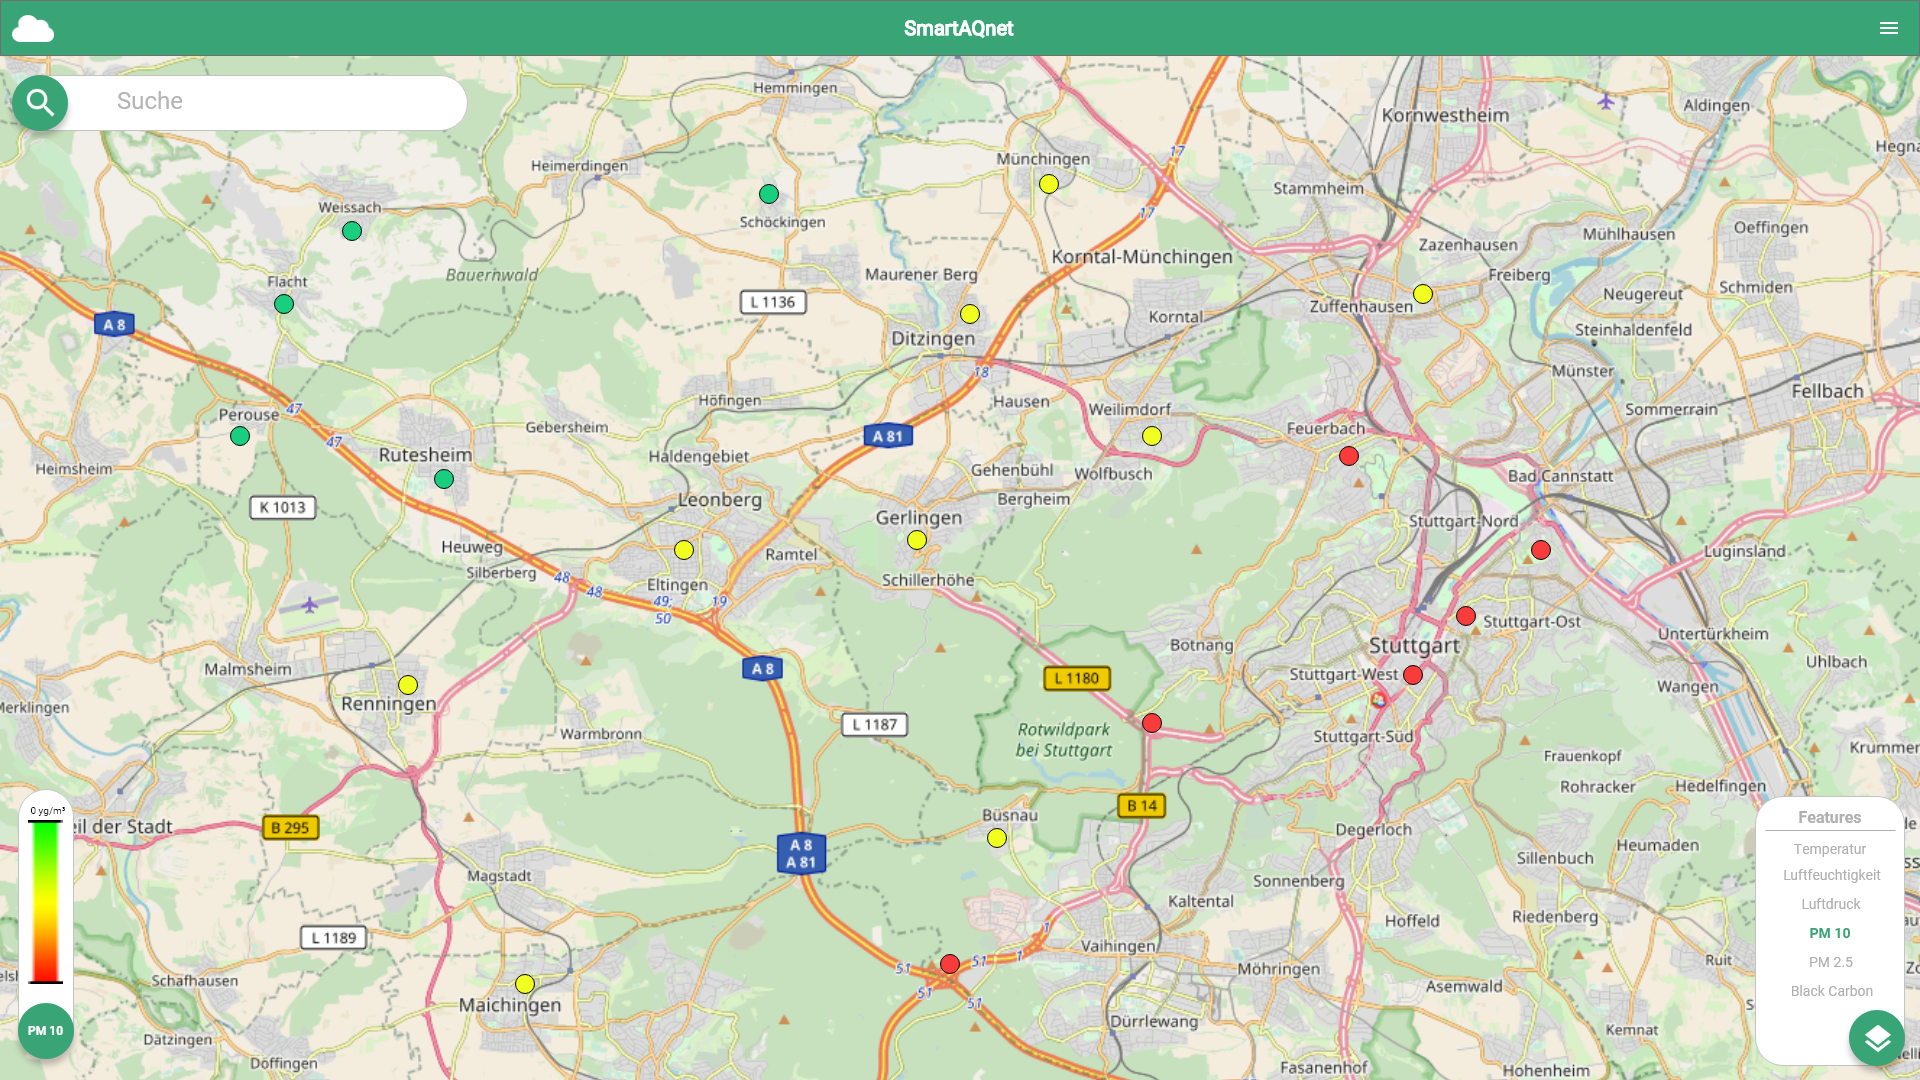
\includegraphics[width=2cm]{Web19202.png}
\noindent\makebox[\textwidth]{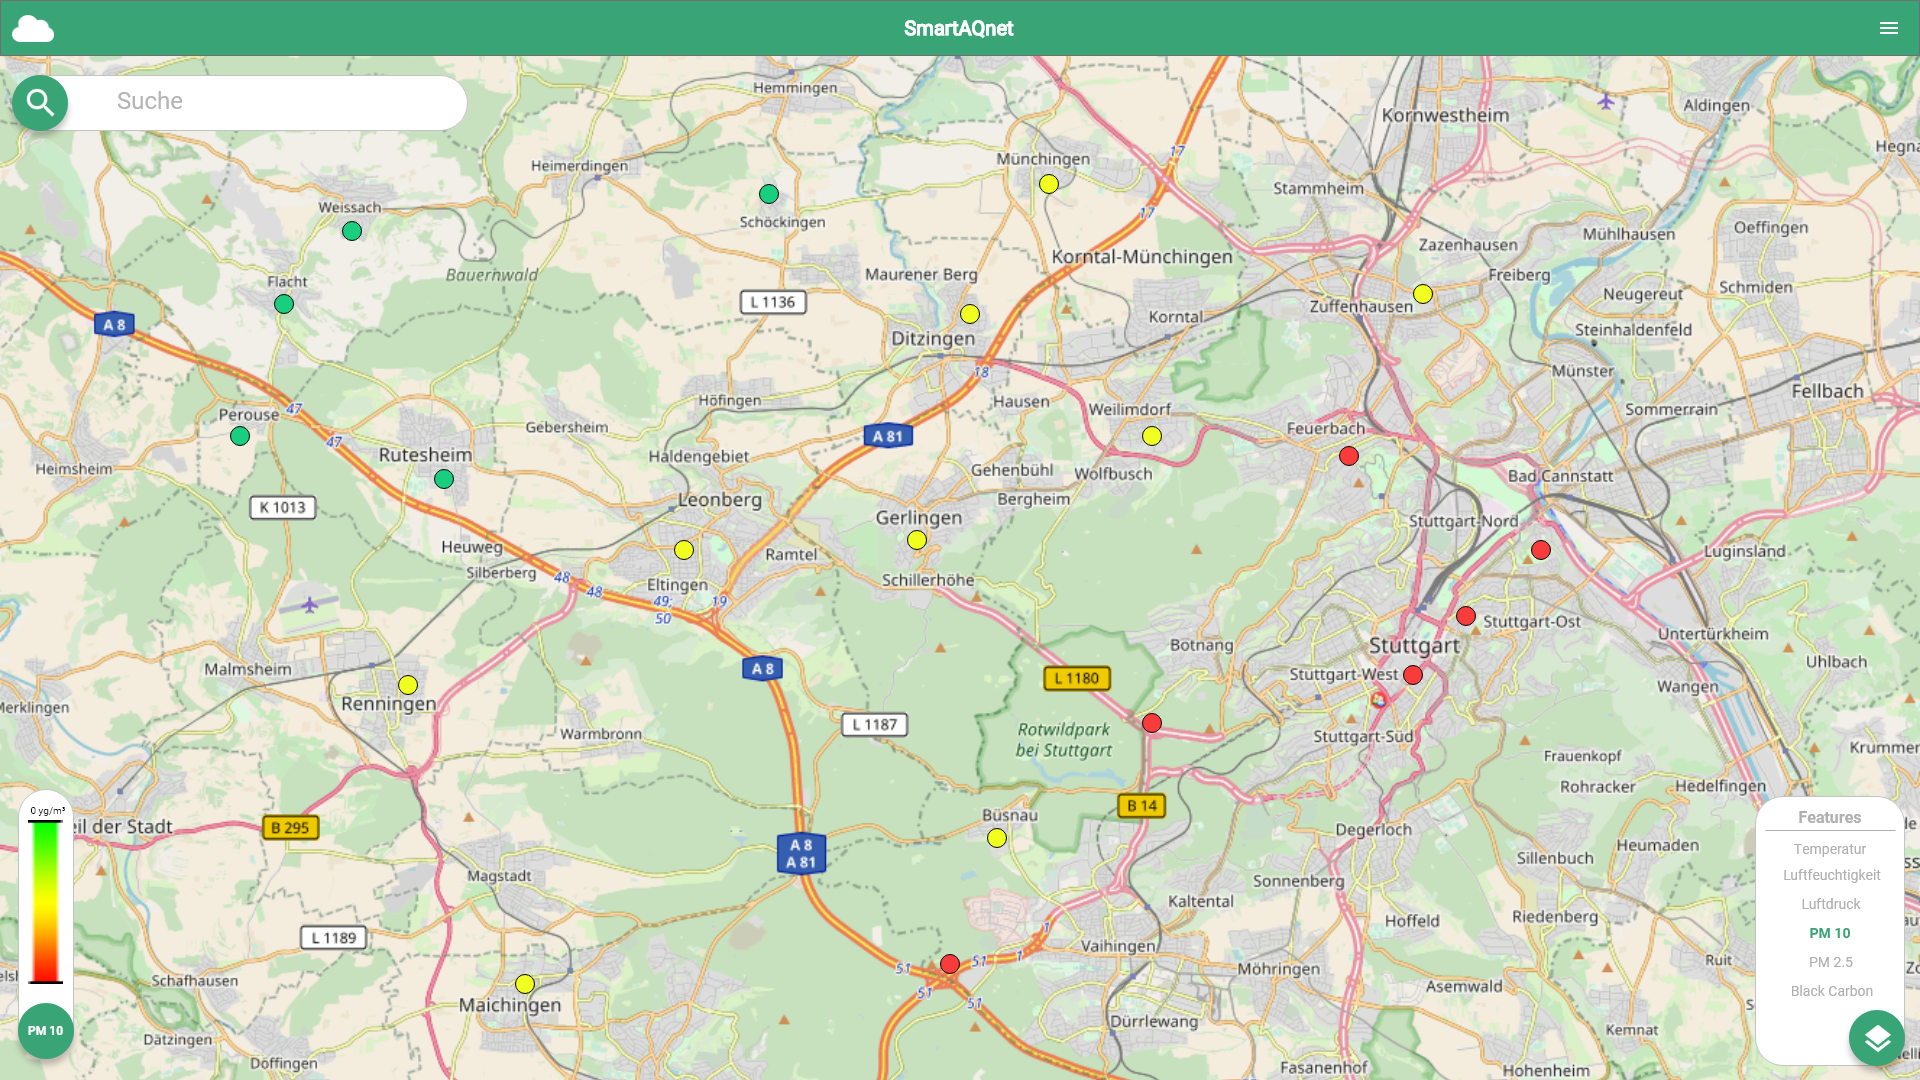
\includegraphics[width=\textwidth]{Web19202.png}}
\noindent\makebox[\textwidth]{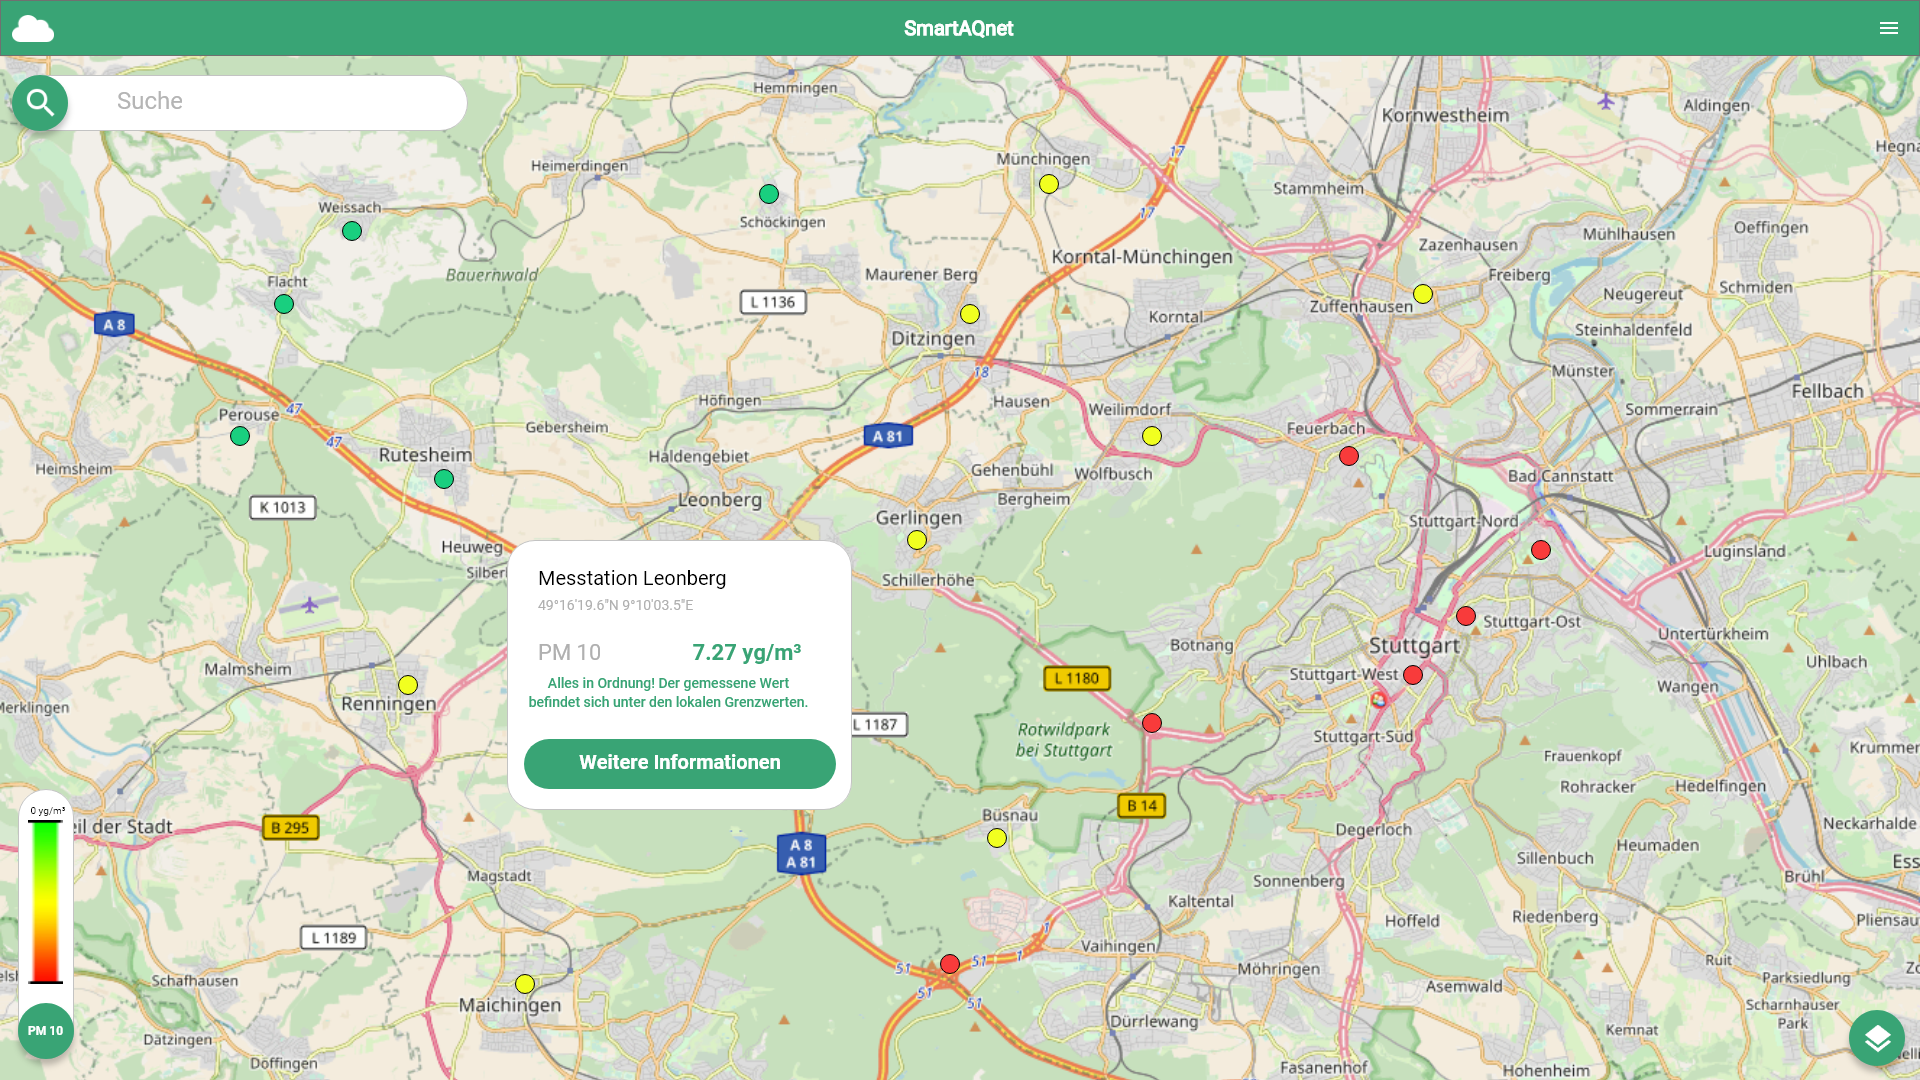
\includegraphics[width=\textwidth]{Web19203.png}}

\section{Entwicklungsumgebung}

\begin{tabular}[htb]{l|r}
    Aufgabe & Software\\
    \hline \hline
    Betriebssystem & Windows 10\\
    \hline
    Textverarbeitung & \LaTeX\\
    TeX-Distribution & MiKTeX/2.9\\
    \LaTeX -Editor & VSCode mit \LaTeX -Erweiterung\\
    \hline
    Versionskontrolle & Git/2.26.2\\
    Remote Repository & GitHub\\
    Git Client & VSCode-Erweiterung\\
    & GitHub Desktop\\
    UML-Tool & dwaw.io\\
    Oberflächenentwurf & Adobe XD\\
    \hline
    Frontend & React/16.13.0 mit TypeScript/3.9.3\\
    Kartenbibliothek React & React Leaflet/2.7.0\\
    React Komponenten Bibiothek & Material UI/4.10.0\\
    React Diagramme & React Google Charts/3.0.15\\
    JavaScript-Paketmanager & npm\\
    Entwicklungsumgebung & VSCode\\
    \hline
    Kommunikation & MSTeams\\
    & WhatsApp\\
    & TECO Mattermost\\
\end{tabular}    

\section{Glossar}

% automatically created glossary (compile twice to show glossary)
\glsaddall
\printnoidxglossaries

% end content
\end{document}